\documentclass{article}

\usepackage{subfig}
\usepackage{tikz}

\usepackage{amsmath}
\usepackage{listings}
\usepackage{algorithm}
\usepackage[noend]{algpseudocode} %for pseudo code, include algorithmicsx automatically

% for better Haskell code outlook
%% \lstdefinelanguage{Haskell}{
%%   basicstyle=\small\ttfamily,
%%   flexiblecolumns=false,
%%   basewidth={0.5em,0.45em},
%%   literate={+}{{$+$}}1 {/}{{$/$}}1 {*}{{$*$}}1 {=}{{$=$}}1
%%            {>}{{$>$}}1 {<}{{$<$}}1 {\\}{{$\lambda$}}1
%%            {\\\\}{{\char`\\\char`\\}}1
%%            {->}{{$\rightarrow$}}2 {>=}{{$\geq$}}2 {<-}{{$\leftarrow$}}2
%%            {<=}{{$\leq$}}2 {=>}{{$\Rightarrow$}}2
%%            {\ .}{{$\circ$}}2 {\ .\ }{{$\circ$}}2
%%            {>>}{{>>}}2 {>>=}{{>>=}}2
%%            {|}{{$\mid$}}1
%% }[keywords,comments,strings]

\lstloadlanguages{C, Haskell, Python}

\lstset{
  showstringspaces = false
}

\begin{document}

\title{The longest palindrome}
\author{Larry LIU Xinyu}
\maketitle

\section{The problem}
A palindrome is a symmetric sequence of elements. It doesn't change when gets reversed.
For example, the English word `madam' is a palindrome. If $S$ is a palindrome, we have
$S = reverse(S)$. Palindrome can be a number, a string, a piece of DNA genome,
or even music. A palindromic sub-string is part of the string that is a palindrome.
For example `issi' is a palindromic sub-string in `Mississippi'. Given a sequence,
there can be
multiple palindromic sub-strings. The problem is to find the longest one.
Take `Mississippi` for example, the longest plindromic sub-string is
`ississi'.

\section{Manacher's algorithm}

There are several methods to solve this problem. The brute-force solution
enumerates all the sub-strings, filters the palindromic ones, and picks the longest.
There are $n(n+1)/2$ sub-strings where $n$ is the length of the string (Empty
string is ignored). The performance of the brute-force method is quadratic.

Another method is to use suffix tree. If $w$ is a palindromic sub-string in
$S$, it must be sub-string of $reverse(S)$ as well.
For example, ``issi'' is a palindromic sub-string of ``Mississippi''
and its reversed form ``ippississiM''.

Based on this fact, we can find the longest palindrome by
searching the longest common sub-string in $S$ and $reverse(S)$.

\begin{equation}
LCS(T_{\textrm{suffix}}(S + reverse(S)))
\end{equation}

Where function $LCS$ finds the
longest common sub-string in the suffix tree in linear time.

The key point is to construct the suffix tree efficiently. There are
some good algorithms achieve the linear time performance, like Ukkonen's algorithm\cite{Ukkonen95}.
This ensures the overall performance of generalised suffix tree method to be linear.

Suffix array provides an easier solution than suffix tree. But it downgrades
the performance to $O(n \lg n)$.

We'll explain a linear time algorithm found by Glenn K. Manacher in 1975 \cite{Manacher75}.
This method scans the string in one round. It reuses the information gained during the scan
which leads to an efficient solution.

For given string $S = \{s_1, s_2, ..., s_n\}$, let $P = \{p_1, p_2, ... p_n\}$ be a table.
$p_i$ is defined as the following.

\begin{equation}
p_i = max \{ d | \{s_{i-d}, ..., s_{i+d}\} \textrm{\ is palindrome}, d = 0, 1, 2, ...\}
\label{eq:p-table}
\end{equation}

We call $P$ the palindrome table.
$p_i$ tells us how long we can extend from the $i$-th element in $S$ to
left and right to form a palindrome. In other words the sub-string
$\{s_{i-p_i}, s_{i-p_i+1}, ..., s_i, ..., s_{i+p_i}\}$ is the longest palindromic sub-string
at the center of $i$. We donote this sub-string as $S_{(i, p_i)}$.
Below table shows an example for string `eneven'.

%\begin{table}
\begin{tabular}{|c|c|c|c|c|c|c|}
\hline
$S$ & e & n & e & v & e & n \\
\hline
$P$ & 0 & 1 & 0 & 2 & 0 & 0 \\
\hline
$S_{(i, p_i)}$ & e & ene & e & neven & e & n \\
\hline
\end{tabular}
%\end{table}

The first value $p_1 = 0$, the palindrome at the center of the first element contains
only one character ``e''. The second value $p_2 = 1$, it means we can extend from
the second element 1 character to both sides. It gives the
palindrome ``ene''. The fourth value $p_4 = 2$, we can extend 2 characters to get
the palindrome ``neven''. We can think
$p_i$ as the `radius' of the palindrome at center $i$.

However, there is a problem in the definition of $p_i$, in equation (\ref{eq:p-table}).
The length of the palindrome is forced to be odd number. It doesn't work
for even length. For example, the $P$ table for string $S = ...issi...$ is as below.

\begin{tabular}{|c|c|c|c|c|c|c|}
\hline
$S$ & ... & i & s & s & i & ... \\
\hline
$P$ & ... & 0 & 0 & 0 & 0 & ... \\
\hline
\end{tabular}

Actually, we need it to be something like this:

\begin{tabular}{|c|c|c|c|c|c|c|c|}
\hline
$S$ & ... & i & s &   & s & i & ... \\
\hline
$P$ & ... &   &   & 2 &   &   & ... \\
\hline
\end{tabular}

One solution is to insert a special delimiter $\# \notin S$ between all elements in $S$ to
turn it into another string $S'$.

\begin{equation}
S' = \{\#, s_1, \#, s_2, \#, ..., \#, s_n, \#\}
\end{equation}

There are two cases.

\begin{itemize}
\item For the odd length palindrome, Let the length be $L = 2k + 1$.

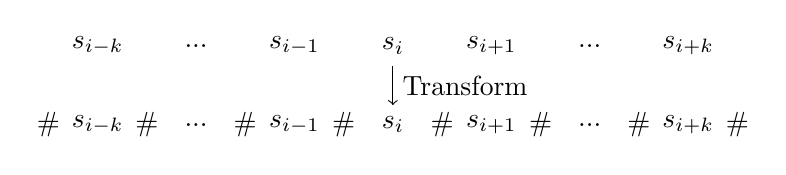
\begin{tikzpicture}[scale=2.5]
  \draw (-1.5cm, .4) node{$s_{i-k}$};
  \draw (-1cm, .4) node{...};
  \draw (-0.5cm, .4) node{$s_{i-1}$};
  \draw (0, .4) node{$s_i$};
  \draw (0.5cm, .4) node{$s_{i+1}$};
  \draw (1cm, .4) node{...};
  \draw (1.5cm, .4) node{$s_{i+k}$};

  \foreach \x in {-1.75, -1.25, ..., 1.75} {
    \draw (\x cm, 0) node{\#};
  }

  \draw (-1.5cm, 0) node{$s_{i-k}$};
  \draw (-1cm, 0) node{...};
  \draw (-0.5cm, 0) node{$s_{i-1}$};
  \draw (0, 0) node{$s_i$};
  \draw (0.5cm, 0) node{$s_{i+1}$};
  \draw (1cm, 0) node{...};
  \draw (1.5cm, 0) node{$s_{i+k}$};

  \draw[->] (0, .3) -- (0, .2) node[right]{Transform} -- (0, .1);

\end{tikzpicture}

After the transformation, the center of the new palindrome is still $s_i$. In the
new palindrome talbe $P'$, the value corresponds to $s_i$ is $p'_j = 2k + 1$.

\item For the even length palindrome, Let the length be $L = 2k$.

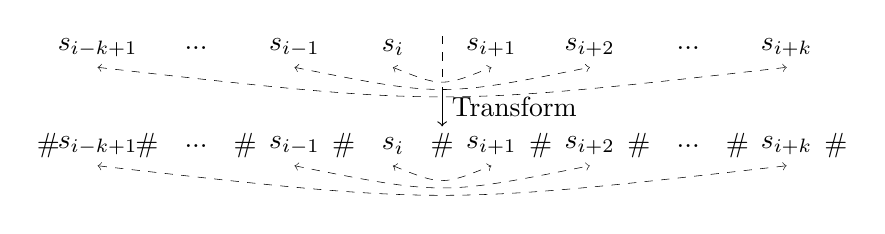
\begin{tikzpicture}[scale=2.5]
  \draw (-1.75cm, .5) node{$s_{i-k+1}$};
  \draw (-1.25cm, .5) node{...};
  \draw (-0.75cm, .5) node{$s_{i-1}$};
  \draw (-0.25cm, .5) node{$s_i$};
  \draw (.25cm, .5) node{$s_{i+1}$};
  \draw (0.75cm, .5) node{$s_{i+2}$};
  \draw (1.25cm, .5) node{...};
  \draw (1.75cm, .5) node{$s_{i+k}$};

  \draw[dashed, very thin] (0, .35) -- (0, .6);
  \foreach \x/\y in {0.25/0.3, 0.75/0.25, 1.75/0.2} {
    \draw[dashed, very thin, <->] (-\x cm, .4) .. controls (0, \y) .. (\x cm, .4);
  }

  \foreach \x in {-2, -1.5, ..., 2} {
    \draw (\x cm, 0) node{\#};
  }

  \draw (-1.75cm, .0) node{$s_{i-k+1}$};
  \draw (-1.25cm, .0) node{...};
  \draw (-0.75cm, .0) node{$s_{i-1}$};
  \draw (-0.25cm, .0) node{$s_i$};
  \draw (.25cm, .0) node{$s_{i+1}$};
  \draw (0.75cm, .0) node{$s_{i+2}$};
  \draw (1.25cm, .0) node{...};
  \draw (1.75cm, .0) node{$s_{i+k}$};

  \foreach \x/\y in {0.25/-0.2, 0.75/-0.25, 1.75/-0.3} {
    \draw[dashed, very thin, <->] (-\x cm, -0.1) .. controls (0, \y) .. (\x cm, -0.1);
  }

  \draw[->] (0, .3) -- (0, .2) node[right]{Transform} -- (0, .1);

\end{tikzpicture}

After the transformation, the center of the new palindrome becomes a delimiter \#. In the
new palindrome talbe $P'$, the value corresponds to the new center is $p'_j = 2k$.
\end{itemize}

In both cases, we have the relationship $L = p'_j$. If we construct a palindrome
table for the transformed string, each value in the table that does not correspond to the delimiter
is the length of the original palindromic sub-string in $S$.
Because the the maximum value in the palindrome table is bound to the longest
one, the problem can be solved with the following strategy:

\begin{enumerate}
\item Transform to a new string with special delimiter interspersed;
\item Construct the palindrome table efficiently;
\item The longest palindromic sub-string can be located by finding the maximum value
in the palindrome table.
\end{enumerate}

\section{The brute-force scan}
The brute-force method scans the transformed string from left to right. For each position
$i$, it checks if $s_{i+k} = s_{i-k}$ for $k = 0, 1, 2, ...$ can be satisfied.

\begin{algorithmic}[1]
\Function{Palindrome}{$S$}
  \State $S' \gets $ empty
  \For{$i \gets 1$ to $|S|$}
    \State $S' \gets S' + \{\#, s_i\}$
  \EndFor
  \State $S' \gets S' + \{\#\}$
  \State $P \gets \{0, 0, ..., 0\}$ \Comment{length of $|S'|$}
  \For{$i \gets 1$ to $|S'|$}
    \While{$1 \leq i \pm p_i \leq |S'|$ and $s'_{i-p_i} = s'_{i+p_i}$}
      \State $p_i \gets p_i + 1$
    \EndWhile
    \State $p_i \gets p_i - 1$
  \EndFor
  \State \Return $max\{p_i\}$
\EndFunction
\end{algorithmic}

The worst case happens when all the characters are same, for instance ``aaa...a'', that
there are $n$ same characters `a'. The brute-force method is quadratic ($O(n^2)$).

\section{Manacher's method}
The key to Manacher's method is information reusing. In order to construct
the palindrome table $P$ efficiently, we need {\em reuse} so far gained result
$p_1 \sim p_{i-1}$ when caculate $p_i$.

Observe the brute-force solution. It compares $s_{i+1}$ with $s_{i-1}$,
$s_{i+2}$ with $s_{i-2}$, ... The element to the right of $s_i$,
may have been examined and it may belong to some previously found palindromic
sub-string. In other words there may be some $j \in [1 \sim i-1]$ that satisfies
$i \leq j + p_j$. This is illustrated in figure \ref{fig:right-most}.
We can record the right most position that the so far found palindromic
sub-strings have riched:

\begin{equation}
r_m = max \{ j + p_j, j < i\}
\end{equation}

\begin{figure}[htbp]
\centering
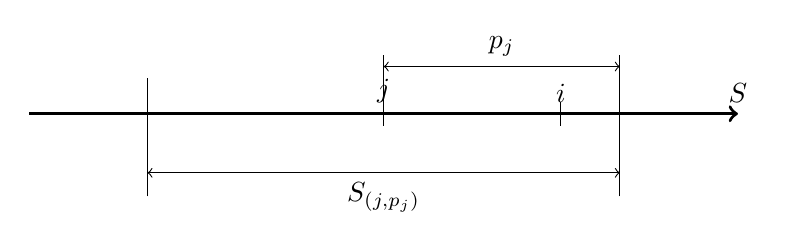
\begin{tikzpicture}[scale=1.5]
  \draw[->, very thick] (-3, .5) -- (0, .5) node[above]{$j$} -- (1.5, .5) node[above]{$i$} -- (3, .5) node[above]{$S$};
  \draw[<->] (-2, 0) -- (0, 0) node[below]{$S_{(j, p_j)}$} -- (2, 0);
  \draw[thin] (-2, -0.2) -- +(0, 1);
  \draw[thin] (2, -0.2) -- + (0, 1.2);
  \draw[thin] (0, 0.4) -- + (0, 0.6);
  \draw[thin, <->] (0, .9) -- +(1, 0) node[above]{$p_j$} -- ++ (2, 0);
  \draw[thin] (1.5, 0.4) -- + (0, 0.2);
\end{tikzpicture}
\caption{Element at $i$ belongs to palindrome $S_{(j, p_j)}$. The palindrome extends to the right of $i$.}
\label{fig:right-most}
\end{figure}

When scan to the $i$-th position from left, we firstly compare $i$ with $r_m$ to check if this position
has been examined before, so that we can reuse the $p_1 \sim p_{i-1}$ information. There are two cases:

\subsection*{Case 1, $i > r_m$}

Because $i > max \{j+p_j, j < i \}$, $s_i$ doesn't belong to any known palindromes. What we can do is as
same as the brute-force method. Scan and compare the symmetric elements $s_{i+k}$ and $s_{i-k}$ until we
find an unmatch. The farest $k$ is the value of $p_i$.

\begin{algorithmic}[1]
\If{$i > r_m$}
  \State $p_i \gets 0$
  \While{$s_{i+p_i} = s_{i-p_i}$}
    \State $p_i \gets p_i + 1$
  \EndWhile
  \State $p_i \gets p_i - 1$
\EndIf
\end{algorithmic}


\subsection*{Case 2, $i \leq r_m$}

Because $i \leq max \{j + p_j, j < i\}$, $s_i$ belongs to some known palindrome. There are three sub-cases:

\subsubsection*{Sub-case 1}

As shown in figure \ref{fig:subcase1}, Denote the $j$ leading to $r_m$ as $j_m$. The palindrome at the
center of $j_m$ is $A = S_{(j_m, p_{j_m})}$. The two elements out of the bound of $A$ are different.
They are represented as $x$ and $y$, $x \neq y$. Because element at $i$ belongs to the palindrome
at the center of $j_m$, its symmetric position to $j_m$ is $2j_m - i$. This is because
$\frac{i + (2j_m -i)}{2} = j_m$. Denote the palindrome at the center of this position as $B$.
In sub-case 1, the left bound of $B$ is to the left of $A$.

\[
left(B) < left(A)
\]

This tells us that $x \in B$. According to the definition of palindrome, there must be a symmetric
element $x'$ in $B$, that $x' = x$. Because $x' \in A$, again, there must be a symmetric element
$x''$ in palindrome $A$, so that $x'' = x$. Since $x \neq y$, we have $x'' \neq y$, this means that
the `radius' of the palindrome at the center of $i$ is equal to the distance between points $a$ and $b$.

\[
r = |a - b| = j_m + p_{j_m} - i
\]


\begin{figure}[htbp]
\centering
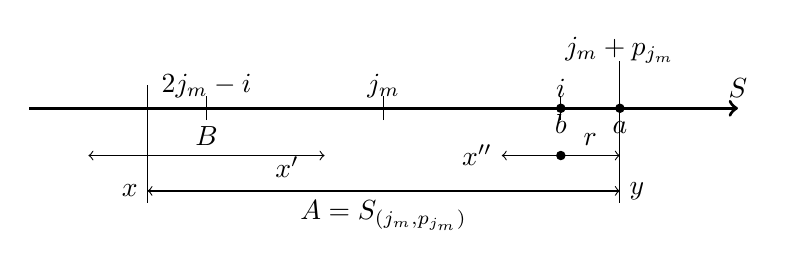
\begin{tikzpicture}[scale=1.5]
  \draw[->, very thick] (-3, .5) --(-1.5, .5) node[above]{$2j_m - i$} --
         (0, .5) node[above]{$j_m$} -- (1.5, .5) node[above]{$i$} --
         (3, .5) node[above]{$S$};
  \draw[thin] (1.5, 0.4) -- + (0, .2); %tick for i
  \draw[thin] (-1.5, 0.4) -- + (0, .2); %tick for 2j_m - i
  \draw[thin] (0, 0.4) -- + (0, .2); %tick for j_m

  % label a, b
  \draw (1.5, .2) node[above]{$b$} (2, .2) node[above]{$a$}
        (2, .8) node[above]{$j_m + p_{j_m}$};
  \filldraw (1.5, .5) circle [radius=1pt]
            (2, .5) circle [radius=1pt];

  % palindrome A
  \draw[<->] (-2, -0.2) node[left]{$x$}-- +(2, 0) node[below]{$A = S_{(j_m, p_{j_m})}$} -- (2, -0.2) node[right]{$y$};
  \draw[thin] (-2, -0.3) -- +(0, 1);   %left bound for S[j_m, P_{j_m}]
  \draw[thin] (2, -0.3) -- + (0, 1.2); %right bound for S[j_m, P_{j_m}]

  % palindrome B
  \draw[<->] (-2.5, .1) -- (-1.5, .1) node[above]{$B$} -- (-0.5, .1);
  \draw (-1, 0) node[right]{$x'$};

  % palindrome at i
  \draw[<->] (1, .1) node[left]{$x''$}-- (1.75, .1) node[above]{$r$} -- (2, .1);
  \filldraw (1.5, .1) circle [radius = 1 pt];

\end{tikzpicture}
\caption{$left(B) < left(A)$}
\label{fig:subcase1}
\end{figure}

The result for sub-case 1 is that $p_i = j_m + p_{j_m} - i$.

\subsubsection*{Sub-case 2}

In sub-case 2, palindrome $B$ is within palindrome $A$ as shown in figure \ref{fig:subcase2}.
Denote the two elements next to the bounds of $B$ as $x$ and $y$, $x \neq y$. As illustrated
in the figure, both $x, y \in A$. Their symmetric elements in $A$ are $x'$ and $y'$, $x' \neq y'$.
The palindrome at the center of $i$ are as same as the palindrome at the center of $2j_m - i$.


\begin{figure}[htbp]
\centering
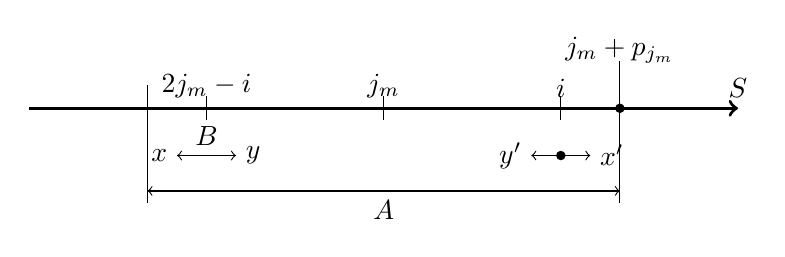
\begin{tikzpicture}[scale=1.5]
  \draw[->, very thick] (-3, .5) --(-1.5, .5) node[above]{$2j_m - i$} --
         (0, .5) node[above]{$j_m$} -- (1.5, .5) node[above]{$i$} --
         (3, .5) node[above]{$S$};
  \draw[thin] (1.5, 0.4) -- + (0, .2); %tick for i
  \draw[thin] (-1.5, 0.4) -- + (0, .2); %tick for 2j_m - i
  \draw[thin] (0, 0.4) -- + (0, .2); %tick for j_m

  % label j_m + p_{j_m}
  \draw (2, .8) node[above]{$j_m + p_{j_m}$};
  \filldraw (2, .5) circle [radius=1pt];

  % palindrome A
  \draw[<->] (-2, -0.2) -- +(2, 0) node[below]{$A$} -- (2, -0.2);
  \draw[thin] (-2, -0.3) -- +(0, 1);   %left bound for S[j_m, P_{j_m}]
  \draw[thin] (2, -0.3) -- + (0, 1.2); %right bound for S[j_m, P_{j_m}]

  % palindrome B
  \draw[<->] (-1.75, .1) node[left]{$x$} -- (-1.5, .1) node[above]{$B$} -- (-1.25, .1) node[right]{$y$};

  % palindrome at i
  \draw[<->] (1.25, .1) node[left]{$y'$} -- (1.75, .1) node[right]{$x'$};
  \filldraw (1.5, .1) circle [radius = 1 pt];

\end{tikzpicture}
\caption{$left(A) < left(B)$}
\label{fig:subcase2}
\end{figure}

This fact indicates the result of sub-case 2 is $p_i = p_{2j_m - i}$.

\subsubsection*{Sub-case 3}

In sub-case 3, palindrome $A$ and $B$ are left aligned as shown in figure
\ref{fig:subcase3}. Denote the two different elements
next to the bounds of $A$ as $x$ and $y$, $x \neq y$. The elements next to
the right bound of $B$ as $y' \neq x$. Because $y' \in A$, its symmetric element in $A$
is $y'' = y'$. But we can't determine if $y$ is equal to $y''$. This tells us
that $p_i$ is at least $p_{2j_m - i}$. We need further scan on both sides
as what the brute-force method does.

\begin{figure}[htbp]
\centering
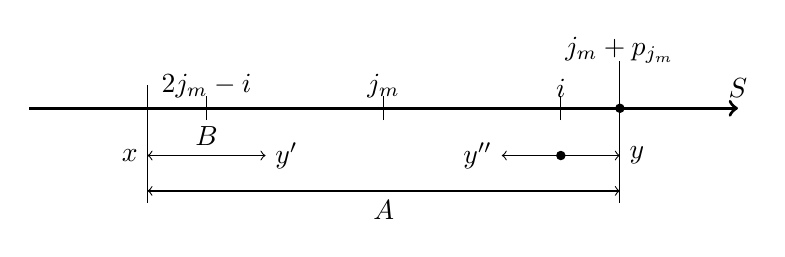
\begin{tikzpicture}[scale=1.5]
  \draw[->, very thick] (-3, .5) --(-1.5, .5) node[above]{$2j_m - i$} --
         (0, .5) node[above]{$j_m$} -- (1.5, .5) node[above]{$i$} --
         (3, .5) node[above]{$S$};
  \draw[thin] (1.5, 0.4) -- + (0, .2); %tick for i
  \draw[thin] (-1.5, 0.4) -- + (0, .2); %tick for 2j_m - i
  \draw[thin] (0, 0.4) -- + (0, .2); %tick for j_m

  % label j_m + p_{j_m}
  \draw (2, .8) node[above]{$j_m + p_{j_m}$};
  \filldraw (2, .5) circle [radius=1pt];

  % palindrome A
  \draw[<->] (-2, -0.2) -- +(2, 0) node[below]{$A$} -- (2, -0.2);
  \draw[thin] (-2, -0.3) -- +(0, 1);   %left bound for S[j_m, P_{j_m}]
  \draw[thin] (2, -0.3) -- + (0, 1.2); %right bound for S[j_m, P_{j_m}]

  % palindrome B
  \draw[<->] (-2, .1) node[left]{$x$} -- (-1.5, .1) node[above]{$B$} -- (-1, .1) node[right]{$y'$};

  % palindrome at i
  \draw[<->] (1, .1) node[left]{$y''$} -- (2, .1) node[right]{$y$};
  \filldraw (1.5, .1) circle [radius = 1 pt];

\end{tikzpicture}
\caption{$A$ and $B$ are left aligned.}
\label{fig:subcase3}
\end{figure}

\begin{algorithmic}[1]
\State $p_i \gets p_{2j_m - i}$
\While{$1 \leq i \pm p_i \leq |S|$ and $s_{i+p_i} = s_{i - p_i}$}
  \State $p_i \gets p_i + 1$
\EndWhile
\State $p_i \gets p_i - 1$
\end{algorithmic}

Summarize the above three sub-cases, we have the following result.

\begin{algorithmic}[1]
\State $p_i \gets min \{p_{2j_m - i}, j_m + p_{j_m} - i\}$
\While{$1 \leq i \pm p_i \leq |S|$ and $s_{i+p_i} = s_{i - p_i}$}
  \State $p_i \gets p_i + 1$
\EndWhile
\State $p_i \gets p_i - 1$
\end{algorithmic}

\section{Manacher's algorithm}

In order to find the length of the longest panlindrome, we intersperse a special delimiter in the string.
Then scan the string to construct the palindrome table. The maximum value
in $P$ gives the final result.

\begin{algorithmic}[1]
\Function{Manacher-Palindrome}{$S$}
  \For{$c \in S$}
    \State $S' \gets S' + \{\#, c\}$
  \EndFor
  \State $S' \gets S' + \{\#\}$ \Comment{Add extra terminator in ANSI C like language}
  \State $P \gets \{0, 0, ..., 0\}$ \Comment{length of $|S'|$}
  \State $j \gets 0, m \gets -\infty$
  \For{$i \gets 1$ to $|S'|$}
    \If{$i \leq j + p_j$}
      \State $p_i \gets min \{p_{2j-i}, j + p_j - i\}$
    \EndIf
    \While{$1 \leq i \pm p_i \leq |S'|$ and $s'_{i+p_i} = s'_{i - p_i}$}
      \State $p_i \gets p_i + 1$
    \EndWhile
    \State $p_i \gets p_i - 1$
    \If{$i + p_i > j + p_j$}
      \State $j \gets i$
    \EndIf
    \State $m \gets max \{p_i, m \}$
  \EndFor
  \State \Return $m$
\EndFunction
\end{algorithmic}

The palindrome table stores enough information about the palindromic sub-strings.
Given $p_j$, The palindrome in the original string $S$ can be expressed as:

\begin{equation}
S[\frac{j-p_j + 1}{2}, \frac{j+p_j-1}{2}]
\end{equation}

When implement this algorithm in programming languages that use left-include-
right-exclude index representation, ANSI C for example, we need adjust
the definition of $p_i$ to simplify the boundary condition. In such environment,
index starts from 0, and end with $n-1$, or expressed as \texttt{s[0..n)}.
It's convenient to use the same idea for the palindrome table. We
define \texttt{p[i]} as the minimum integer that satisifies \texttt{s[i+p[i]]}
$\neq$ \texttt{s[i-p[i]]}. This value is one element longer than what
we defined previously. We needn't decrease it by one after the while-loop.
But we need change the condition when compare $i$ with $r_m$. The length
of the original palindrome changes to \texttt{p[i] - 1} respectively.
The following Python example program implements the Manacher's algorithm.

\lstset{language=Python}
\begin{lstlisting}
DELIMITER = "#"
def manacher_palindrome(s):
    s = DELIMITER + DELIMITER.join(s) + DELIMITER
    n = len(s)
    p = [0] * n
    j = 0
    m = (-1, 0)  # (max length so far, position)
    for i in xrange(n):
        p[i] = min(p[2*j-i], j + p[j] - i) if i < j + p[j] else 1
        while 0 <= i - p[i] and i + p[i] < n and s[i-p[i]] == s[i+p[i]]:
            p[i] = p[i] + 1
        if j + p[j] < i + p[i]:
            j = i
        m = max(m, (p[i] - 1, i))
    return m
\end{lstlisting}

It can report both the length and the content of the longest palindrome like below.

\lstset{language=Python}
\begin{lstlisting}
(n, i) = manacher_palindrome(s)
print "The longest:", s[(i-n+1)/2 : (i+n-1)/2+1], " len:", n
\end{lstlisting}

Manacher's algorithm performs in linear time $O(n)$. This is because for any element $s_i$,
after its first time successful comparison with some other $s_k$, $k < i$, it would never be compared
successfully with any $s_j$, $j < i$. The overal unsuccessful comparison is at most $n$.

\begin{thebibliography}{99}

\bibitem{Ukkonen95}
Esko Ukkonen. ``On-line construction of suffix trees''. Algorithmica 14 (3): 249--260. doi:10.1007/BF01206331. http://www.cs.helsinki.fi/u/ukkonen/SuffixT1withFigs.pdf

\bibitem{Manacher75}
Manacher, Glenn (1975), ``A new linear-time `on-line' algorithm for finding the smallest initial palindrome of a string'', Journal of the ACM 22 (3): 346�C351, doi:10.1145/321892.321896

\bibitem{wiki-longest-palindrome}
Longest palindromic substring. Wikipedia. http://en.wikipedia.org/wiki/Longest\_palindromic\_substring

\end{thebibliography}

\end{document}
